\documentclass[12pt,a4paper,titlepage,twoside]{report}
\usepackage[utf8]{inputenc}
\usepackage[french]{babel}
\usepackage[T1]{fontenc}
\usepackage{amsmath}
\usepackage{amsfonts}
\usepackage{amssymb}
\usepackage{graphicx}
\usepackage{url}
\usepackage[usenames,dvipsnames]{xcolor}
\usepackage[colorlinks=false,urlbordercolor=white,linkbordercolor=white]{hyperref}
\usepackage[left=2cm,right=2cm,top=2cm,bottom=2cm]{geometry}
\usepackage{fancyhdr}
\usepackage{lmodern}
\usepackage{listings}
\pagestyle{fancy}
\usepackage{titlesec}
\usepackage[abs]{overpic}

% Definition des couleurs
\definecolor{titreColor}{RGB}{0,58,128}  % Marine
\definecolor{stitreColor}{RGB}{0,158,224}  % Ocean
\definecolor{auteurColor}{RGB}{0,58,128}     % Marine
\definecolor{texteColor}{RGB}{164,196,0}     % Prairie

% Definition des chapitres
\titleformat{\chapter}[display]
{\normalfont\Large\filcenter\sffamily}
{\titlerule[1pt]%
 \vspace{1pt}%
 \titlerule
 \vspace{1pc}%
 \Large\color{titreColor}{\MakeUppercase{\chaptertitlename} \thechapter}}
{1pc}
{\titlerule
 \vspace{1pc}%
 \Huge}

\titleformat{\section}
{\color{titreColor}\normalfont\Large\bfseries\sffamily}
{\color{titreColor}\thesection}{1em}{}

\titleformat{\subsection}
{\color{stitreColor}\bfseries\sffamily}
{\color{stitreColor}\thesubsection}{1em}{}

%Données de titre et d'auteur pour la page de garde
\newcommand{\titre}{Développement de l'application web USACT}
\newcommand{\sousTitre}{Stage de DUT Informatique réalisé par \newline Jérémy DAMEY \newline Du 7 avril au 12 juin 2015}
\newcommand{\auteur}{Jérémy DAMEY}
\newcommand{\dateModif}{\today}

\begin{document}
%Supprime les veuves et orphelines
\widowpenalty=10000
\clubpenalty=10000
\raggedbottom 

% Integre la page de garde
%\input{title.tex}
\underline{Maître de stage :} Eric QUINTON \hspace{2cm}
\underline{Enseignant referent :} Franck RUBI 
\input{Page_de_garde}
% Définition des entêtes
\fancyhead{}
\fancyhead[CO]{\leftmark\sffamily}
\fancyhead[CE]{ \sffamily\titre{}}
\fancyfoot[CO]{\sffamily\thepage}
\fancyfoot[CE]{\sffamily\thepage}
% Redéfinition de \cleardoublepage pour créer une page vide
\makeatletter
\def\cleardoublepage{\clearpage\if@twoside \ifodd\c@page\else
  \hbox{}
  \vspace*{\fill}

  \vspace{\fill}
  \thispagestyle{empty}
  \newpage
  \if@twocolumn\hbox{}\newpage\fi\fi\fi}
\makeatother

% \cleardoublepage permet de générer une page vide 
% si le chapitre ne commence pas sur la page de droite
\cleardoublepage
\vspace{1cm}
\begin{center}
\bf 
\color{titreColor}
\LARGE{Résumé :}
\end{center}
J'ai effectué mon stage au sein de l'IRSTEA (enseignement appelé Cemagref) situé à Cestas-Gazinet du 7 avril au 12 juin. L'IRSTEA s'occupe de recenser les conflits qu'il y a au sein de l'estuaire de la gironde. Pour faciliter ce travail aux chercheurs au moment de la consultation et de la saisie d'un conflit, il leur faut un logiciel. \newline

L'objectif de mon stage a été de recréer intégralement la base de données en PostGreSQL qui été déjà existante au format ACCESS. J'ai dû également crée l'application web en PHP permettant de pouvoir afficher les conflits ainsi que la saisie de nouveau tout en respectant une certaine ergonomie. \newline

Dans mon rapport, je parlerais de ce qui était déjà existant ainsi que de l'application web que j'ai crée.

\vspace{1cm}
\begin{center}
\bf 
\color{titreColor}
\LARGE{Abstract :}
\end{center}
I did my placement in IRSTEA (teaching called Cemagref) located in Cestas-Gazinet from April 7 to June 12. The IRSTEA handles identify conflicts that there are in the estuary of the Gironde. To facilitate this work to researchers at the time of consultation and the seizure of a conflict, they need software. \newline

The goal of my placement was fully recreate the database in PostgreSQL that was existing in ACCESS format. I had also creates the PHP web application that can view the conflict as well as the new entry while maintaining a certain ergonomics. \newline

In my report, I would talk about what was already existing as well as the web application that I created.

\cleardoublepage
\vspace{1cm}
\begin{center}
\bf 
\color{titreColor}
\LARGE{Remerciements :}
\end{center}
Tout d'abord, je tiens à remercier mon maître de stage Eric QUINTON pour m'avoir accepté au sein de l'IRSTEA et pour tout ce qu'il m'a apporté durant la durée de ce stage. \newline\newline
Je remercie également les chercheuses Sandrine LYSER et Clarisse CAZALS pour leurs disponibilités et les éclaircissements qu'elles m'ont apportés pendant ces 10 semaines. \newline\newline
Je tenais également à remercier l'IRSTEA pour l'accueil chaleureux que j'ai reçu. \newline\newline
Enfin, je remercie mes professeurs pour tout ce qu'ils m'ont apporté au cours de ces 3 années de formation. 

\cleardoublepage
\setcounter{tocdepth}{4}
\tableofcontents
\clearpage
\listoffigures

\cleardoublepage
\chapter{Introduction}
Irstea, institut de recherche en sciences et technologies pour l’environnement et l’agriculture, est un établissement public de recherche dans le domaine de l’environnement et de l’agriculture. Son unité de recherche Environnement, territoires et infrastructures (ETBX) est chargée, pour une partie de ses activités, de développer des recherches sur les dynamiques territoriales en lien avec le renouvellement des enjeux environnementaux et le changement climatique. C’est au sein de cette unité que j’ai effectué mon stage de DUT informatique pour une durée de 10 semaines sous la responsabilité de Eric QUINTON. \newline

Le conflit est l'expression d'un problème entre 2 ou plusieurs acteurs dans une zone géographique bien délimitée dans un domaine d'étude précisé. Pour faciliter la saisie et la consultation d'un conflit, USACT, une application PHP, a été développée en 2010. Cet outil, couplé à une base de données PostGreSQL, permet la saisie et la consultation des données se rapportant aux conflits. Cependant, depuis sa dernière version, des modifications se sont révélées être nécessaires. \newline


Dans un premier temps, je présenterais l'institut de recherche IRSTEA. Ensuite, je resituerais le contexte du stage ainsi que les outils utilisés. Enfin, je parlerais de l'étude du sujet et des tâches que j'ai effectuées durant ce stage.

\cleardoublepage
\chapter{Présentation de l'IRSTEA}
\section{Linstitut de l'IRSTEA}
Auparavant appelé Cemagref, l’IRSTEA (Institut national de Recherche en Sciences et Technologies pour l’Environnement et l’Agriculture) est un organisme de recherche. \newline\newline
Cet organisme travaille sur les enjeux majeurs d’une agriculture responsable et de l’aménagement durable des territoires ainsi que de la gestion des eaux et des risques qui leur sont associés (sécheresse, inondation …). Tous les ingénieurs et les chercheurs travaillent chaque jour pour accomplir leur mission : relever le défi de la compréhension du changement global pour un développement durable et éco-responsable. \newline
Au sein des neuf centres régionaux, les chercheurs d'IRSTEA sont en prise directe avec les territoires, sur l'observation desquels ils fondent leurs recherches. \newline\newline
La science environnementale offre en effet une étroite imbrication entre expérimentation, modèles théoriques et innovation technologique et se traduit par un partenariat étroit avec les acteurs publics et le tissu économique. 

\section{L'IRSTEA à Bordeaux}
Le centre de recherche de Bordeaux est l’une des neuf implantations d'Irstea. Localisé sur le site principal de Cestas – Gazinet, ses activités de recherche, d’appui aux politiques publiques et d’expertise portent sur 2 domaines principaux : la gestion de l’eau et du fonctionnement des milieux aquatiques et l’interface entre eau et gestion des territoires. \newline\newline
Ses recherches sont effectuées en collaboration avec des laboratoires publics français ou européens (Université de Bordeaux, Université de Pau, CNRS, INRA ...) et des entreprises ou bureaux d’études privés. \newline\newline
Au sein du centre de Bordeaux, il y a deux unités de recherche :
\begin{description}
\item[- Ecosystèmes aquatiques et changements globaux (EABX) : ]Cette unité axe ses actions de recherche et d’expertise sur l’eau, sur la qualité des hydrosystèmes continentaux et sur l’appréciation de l’état et de la dynamique de fonctionnement des milieux et espèces susceptibles d’agir sur les édifices biologiques (pêche, perturbations, obstacles, contamination, changements environnementaux),
\item[- Environnement, territoires et infrastructures (ETBX) : ] Cette unité développe des recherches sur les dynamiques territoriales en lien avec le renouvellement des enjeux environnementaux et le changement climatique.\newline
\end{description}
Ci-dessous, l'organigramme de l'unité ETBX (figure 1). J'ai intégré l'équipe EADT (Environnement, Acteurs et Dynamiques Territoriales). \newline

\begin{figure}[!ht]
\center
\includegraphics[width=12cm,height=12cm,keepaspectratio]{Image/Organigramme_UR_ETBX}%
\caption{Organigramme de l'unité ETBX} 
\label{Organigramme de l'unité ETBX}
\end{figure}



\begin{tabbing}
Voici \= quelques chiffres sur les effectifs de Bordeaux : \\
\> - 2 unités de recherche \\
\> - 1 équipe services généraux et appui à la recherche \\
\> - 180 personnes dont la moitié de chercheurs et d'ingénieurs \\
\> - En moyenne 20 doctorants et post-doctorants par an \\
\> - Entre 30 et 35 agents en Contrat à Durée Déterminée \\
\> - Entre 25 et 30 stagiaires de l'enseignement supérieur \\
\> - 7 millions d'euros de budget annuel (hors salaires personnel permanent), dont 70 \% provenant \\ 
\> de ressources propres par contrats de recherche ou transferts. \newline\newline
\end{tabbing}

L'équipe EADT travaille sur la gestion des conflits au sein du basin d'Arcachon. Par la suite, nous allons voir les cas d'utilisations que j'ai établis avant de vraiment commencé la réalisation du projet. Ensuite nous verrons les nouveaux outils que j'ai utilisé et leur fonctionnement. Enfin, nous verrons à quoi ressemble le logiciel. 


\cleardoublepage
\chapter{Le contexte du stage}
\section{Le conflit}
Un conflit est un combat, une lutte armée entre deux ou plusieurs personnes ou puissances qui se disputent un droit. Au sens figuré, c'est une violente opposition de sentiments, d'opinions ou d'intérêts, un antagonisme entre des forces contraires. \newline

Un intérêt est ce qui importe à quelqu'un, ce qui lui convient, ce qui lui procure un avantage, une utilité. C'est aussi le profit tiré par un prêteur, sous la forme d'une rémunération de l'argent prêté à un emprunteur.\newline

Voici donc 2 définitions permettant de définir un conflit.
Dans le cadre de l'IRSTEA, un conflit est l'expression d'un problème entre 2 ou plusieurs acteurs dans une zone géographique bien délimitée dans un domaine d'étude précisé. 

\begin{tabbing}
Un \= conflit est identifié par : \\
\> \textbf{- Les sources de données :} informations sur la source de données \\
\> \textbf{- Les matériels du conflit :} informations sur le bien support, l'objet du conflit \\
\> \textbf{- Le genèses et déroulements du conflit :} période, localisation, résolution \\
\> \textbf{- Les acteurs du conflit :} informations sur les personnes (physiques et/ou morales) qui \\
\> participent au conflit \\
\> \textbf{- Les interventions des acteurs dans le conflit :} rôle de l'acteur, lien avec la matérialité du \\ 
\> conflit, motifs de revendication et types d'arguments invoqués, mode d'action, solution proposée \\
\end{tabbing}

Ci-dessous \textit{(figure 2.1)}, vous trouverez un diagramme expliquant le déroulement d'un conflit avec plusieurs source d'informations relatant du conflit. Une fois que le conflit est déclaré, nous avons la décision de justice, c'est-à-dire celle qui va donné le verdict annoncé. \newline
Enfin, nous avons les personnes qui subissent le conflit, autrement dit les personnes où la décision annoncé par la justice n'a pas été en leur faveur. Nous avons également une administration qui est prise à partie pour énoncer un autre avis.

\clearpage
\begin{figure}
\centering
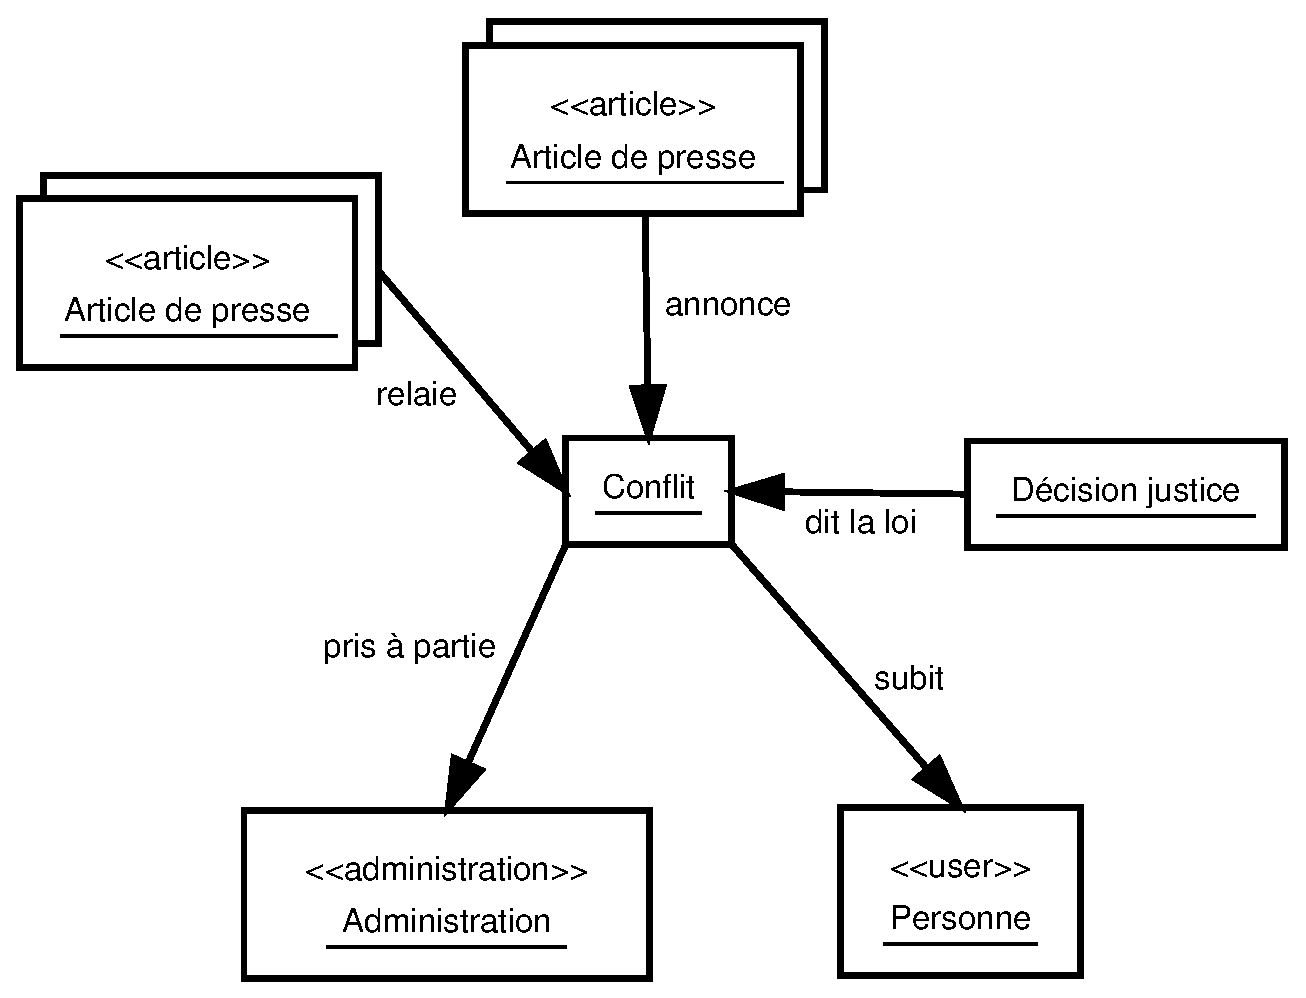
\includegraphics[width=\textwidth]{Image/ExplicationConflit.eps}
\caption{Diagramme de la description d'un conflit}
\end{figure}

Pour faciliter la déclaration d'un conflit, nous avons mis en place une application web appeler USACT permettant la saisie de celui-ci.

\section{USACT situation initiale}
Cette application a été, initialement, conçu pour gérer les conflits d'usage au sein du bassin d'Arcachon. L’étude des conflits s’appuie sur une méthodologie développée par Torre et al. (2010), \emph{comment évaluer et mesurer la conflictualité liée aux usages de l'espace ? Eléments de méthode et de repérage.} \newline \newline

L'étude des conflits est basée sur l’utilisation de trois sources de données complémentaires :
\begin{description}	
\item[–	La Presse Quotidienne Régionale  (PQR) ,] pour accéder à une information locale détaillée;
\item[–	Les entretiens auprès d’experts ,] pour recueillir des informations auprès d’experts locaux, impliqués ou non dans les conflits; 	
\item[–	Les relevés de contentieux ,] permettant de recenser les conflits qui font l’objet d’un  traitement juridique. \newline\newline
\end{description}

Initialement créée sous ACCESS, la base de données a été migrée vers un serveur de base de données en PostGreSQL. L’interface de saisie est alors devenue inadaptée. Le but est de faciliter l’accès aux données pour les chercheurs impliqués dans un projet. L'objectif est qu'il est l'accès aux données en lecture et en écriture. \newline \newline

Les données sont organisées en domaine d'études, c'est-à-dire en zone géographique restreinte et homogène pour étudier les conflits d'usage. L'application devra permettre aux chercheurs de travailler dans trois domaines : Arcachon, Marseille et l'Île de la Réunion.

\section{Outils utilisés}
\subsection{SMARTY}
Le principale outil que j'ai utilisé est le moteur de template PHP Smarty. \newline\newline
Un moteur de template PHP est écrit en PHP. Son rôle est principalement de vous aider dans la lisibilité et la logique de votre projet en général, de son code en particulier. Également couplé d'une structure MVC, ce système donne d'excellentes performances. \newline
Ce que fait précisément un moteur de template, c'est rassembler le code de présentation (tout ce qui est (x)HTML et CSS) et le code d'application (votre requête en PHP et autres). \newline
Ainsi, plus besoin de se casser la tête à retrouver la requête dans la structure HTML du site ou encore à rechercher la variable dans un monticule de texte. \newline\newline

Le rouage d'un moteur de template est bien huilé. En effet, prenons une page d'index contenant une série de news. Le fichier PHP va se charger de rechercher les informations dans la base de données : titre, contenu, créateur… \newline
Ce fichier ne contient aucune balise (x)HTML ayant une influence sur l'affichage. Et d'un autre côté, on trouve un fichier de template (.html ou .tpl) qui contient la structure (x)HTML de la page web. Grâce au moteur de template, les informations contenues dans le fichier PHP lui seront transmises et le moteur regroupera les deux fichiers en un seul par une compilation. \newline

\begin{tabbing}
Voici \= comment fonctionne la compilation complète des deux fichiers : \\
\> - lecture du fichier PHP ; \\
\> - lecture du template ; \\
\> - compilation ; \\
\> - création du script PHP à partir des deux autres ; \\
\> - exécution du code généré. \\
\end{tabbing}

Bien sûr, un tel système comprend son lot d'avantages, mais aussi d'inconvénients. \newline

\begin{flushleft}
\bf
Les avantages :
\end{flushleft}
\begin{description}
\item[ - ] La séparation des deux codes permet une meilleure visibilité dans le code. Idéal pour le travail d'équipe. 
\item[ - ] On peut alors toucher ou modifier un des deux fichiers sans que cela ait un impact sur l'autre. 
\item[ - ] La mise en cache est proposée et permet ainsi d'économiser les ressources des serveurs avec la possibilité de configurer le tout. 
\end{description}

\begin{flushleft}
\bf
Les inconvénients :
\end{flushleft} 
\begin{description}
\item[ - ] Son utilisation va retarder le chargement de votre page, mais il sera compensé en partie par Smarty, un moteur de template assez rapide.
\item[ - ] Il faut étudier le langage de template.
\item[ - ] La lecture des erreurs est assez compliquée. \newline
\end{description}

Smarty, moteur de template, est donc celui que j'ai décidé de vous présenter pour ses capacités très puissantes et son utilisation très facile pour les débutants. Il a l'avantage d'être très rapide : Smarty recompile les fichiers uniquement si des changements sont apportés dans le fichier de template. 

\subsection{Les autres outils}
USACT a été programmé en PHP sous l’IDE (Integrated Development Environment) \textit{Eclipse}. Un IDE est une interface de développement qui permet de programmer. \newline
Sur un même IDE nous pouvons utiliser de multiples langages différent les uns des autres. Par exemple Eclipse est utilisé pour le PHP mais nous pouvons également faire du Java, du python... \newline\newline

Toutes les informations sont stockées dans une base de données PostGreSQL. Par le biais de requête SQl nous pouvons interroger la base pour afficher la liste des conflits, nous pouvons également supprimer ou modifier les conflits sélectionner. \newline
Pour interagir avec la base nous avons utiliser le logiciel SQLWorkbench. \newline
Pour faire des schémas de la base de données, j'ai utilisés le logiciel SQl Power Architect. Il permet, dès que le schéma de la base est réalisé, de produire un script SQL que nous exécutons directement depuis SQLWorkbench.\newline\newline

Pour tout ce qui touche au versionning, j'ai utilisé GIT en passant par la Forge (logiciel interne à l'IRSTEA ayant les mêmes fonctionnalités que GitHub). \newline\newline

Enfin, pour tout ce qui est rédaction de rapport (y compris le rapport de stage), j'ai utilisé le LaTex avec le logiciel TexMaker qui compile le fichier .tex et qui génère directement le fichier final au format PDF. \newline




\cleardoublepage
\chapter{Les tâches effectuées}
\section{Étude du sujet}
Dans un premier temps, mon rôle a été de comprendre ce que j'avais à faire. Au tout début, j'ai eu une réunion avec les chercheurs pour savoir précisément leur attentes pour le développement de l'application. \newline
J'ai donc commencer par établir les cas d'utilisations possible pour bien assimiler le sujet et pour également me permettre de savoir si j'avais bien compris leur attentes. Dès que j'avais une version présentable, j'allais voir mon maitre de stage pour avoir son avis. J'ai répété ce geste jusqu'à ce que j'ai une version du rapport des cas d'utilisations correcte. \newline\newline

Mes cas d'utilisations étaient présenter en 2 parties. Il y avait une première partie présentation du problème. C'est la partie qui permet de ressituer le contexte, à savoir ce qui est déjà existant en terme d'application. On rappelle également comment est étudier un conflit qui est la partie primordiale de mon sujet de stage. \newline
Dans une deuxième partie, j'ai fait un schéma général des cas d'utilisations et par la suite j'ai expliqué chaque cas d'utilisation en précisant bien le but de chacun et en ajoutant des définitions des mots technique et important si cela était nécessaire. \newline
Mes parties importante étaient de bien comprendre comment on identifier un conflit mais aussi comment extraire les données relatant des conflits. \newline\newline

Pour faire le point sur l'étude du sujet et de sa compréhension, j'avais une réunion tout les matins avec mon maitre de stage. J'avais également une réunion toutes les 3 semaines environ pour faire un point plus détaillé avec cette fois-ci la présence des chercheurs. \newline\newline

Dans un deuxième temps, j'ai crée la base de données qui permet de stocker toute les informations se rapportant aux conflits que nous allons voir par la suite.


\clearpage
\section{Création de la base de données}
Après avoir étudier complètement le sujet, je me suis attaqué à la partie base de données. C'est la partie la plus importante du projet étant donné que cela constitue la base principale. S'il n'y a pas de base de données, on ne peut pas passer à la phase de développement. Une base de données est déjà existante sous Access. Elle contient 22 tables. \newline\newline

Mon but était de la refaire en PostGreSQL en respectant les normes adéquat. Par conséquent, j'ai du repenser toute la base en commençant par l'interroger pour savoir ce que contenait chaque table. J'ai casé toute la base en rajoutant de nouvelles tables, en renommant certaine table ainsi que les attributs pour respecter toutes les normes PostGreSQL. \newline
Pour ne pas faire dans la précipitation et pour rendre un travail propre, je refait la base de données pas à pas. Je commence par la tables la plus importante et je rajoute au fur à mesure. Pendant la durée de mon stage, je me suis attaqué à 6 tables sur les 22 existantes dans la base Access, à savoir les tables en rouge (CONFLITSEXPR et CONFLITS) ainsi que les tables orange (INTERVENTIONS, MODESACTION, REVENDICATIONS et ACTEURS). Vous trouverez la base complète en annexe. \newline\newline

Dans la nouvelle base que j'ai intégralement repensé, il y a actuellement 33 tables. Je vais vous présenté le rôle de chacune d'elles. La table CONFLITSEXPR a été renommé en CONFLIT (représenté en jaune sur le schéma). Le contenu de la table est identique. La table CONFLITS a été renommé en PERIMETRE (représenté en rose sur le schéma). Pour respecter les normes et pour rendre le schéma plus compréhensible, j'ai du diviser cette table en plusieurs tables (ce sont toutes les tables représenter en rose). Ce sont les 2 tables principales du projet, c'est donc ces tables que j'ai repensé en premier.\newline
Ensuite, je suis passé à la table ACTEURS qui était une grosse table. J'ai passé du temps dessus. Par conséquent, elle a également été divisé en plusieurs tables également. C'est aussi une table importante car il y a toujours un ou plusieurs acteurs qui interviennent dans un conflit. Sur le nouveau schéma, la table s'appelle ACTEUR (représenté en violet). \newline
Enfin, je suis passer à la table INTERVENTIONS et les tables MODESACTION et REVENDICATIONS pour pouvoir relier les acteurs aux conflits.  la table INTERVENTIONS s'appelle INTERVENTION (en bleu clair sur le schéma). C'est donc cette table qui permet d'assurer la liaison. Les tables MODESACTION et REVENDICATIONS sont seulement relier a la table INTERVENTIONS, c'est pour cela que je les ai intégré sur le schéma. \newline\newline

Pour le développement de l'application web, je me suis intéressé aux tables CONFLIT et PERIMETRE. Cela permet d'avoir la base de l'application opérationnel. C'est ce que nous allons voir par la suite.

\clearpage
\section{Application web}
Dans cette partie, je vais parlé de la partie principale de mon stage, à savoir la réalisation de l'application web USACT. Le but de cette application est de pouvoir saisir un conflit, afficher la liste des conflits existant, pourvoir rechercher un conflit précis avec des critères de recherches et enfin pouvoir modifier un conflit.\newline
Je vais donc détaillé chaque module de l'application avec leur rôle.\newline\newline

Je vais commencé par parler des paramètres, c'est-à-dire ce qui correspond aux tables de paramètre dans la base de données.

\section{Tâches réalisées}
Pendant ce stage, j'ai effectué de nombreuses tâches. Tout d'abord, j'ai commencé par l'apprentissage des nouveaux logiciel pour avoir une bonne prise en main par la suite. Que ce soit des logiciels de base de données, de conception ou de rédaction de rapport, tout y est passé. \newline\newline

Ensuite, j'ai rédiger le rapport des cas d'utilisations se rapportant au projet USACT, pour pouvoir avoir un fil directeur pour la suite du stage et surtout pour le développement de l'application web.\newline\newline

Après je suis passé à la création de la base de données en PostGreSQL en me basant sur celle déjà existante sous Access. Je rajoutais les tables au fur et à mesure, dès que cela était utile et pertinent. \newline\newline

Enfin, j'ai développé l'application web USACT comme expliqué dans la partie précédente.


\cleardoublepage
\chapter{Conclusion}
Ce stage de 10 semaines m’a permis de réaliser mon premier projet dans le monde professionnelle au sien de l'Irstea, qui concerne la saisie d'un nouveau conflit. Ce projet étant assez conséquent, je n'ai pas eu le temps de le mener à bout. Il faudrait environ un mois supplémentaire pour pouvoir mener ce projet à bien. \newline\newline

A l’issu de ce stage, la saisie d'un conflit est opérationnelle. On peut également associer le périmètre correspondant au lieu où s'est déroulé le conflit. \newline\newline

Ce stage m'a permis de développer de nouveau acquis tel que le moteur de template Smarty et dans consolider certains comme le pattern MVC (Modèle Vue Controller). Par la même occasion, le fait de develloper un logiciel pour des professionnels nous met une pression supplémentaire et cela nous incite à rendre un travail propre et opérationnelle. \newline\newline

Le fait de travailler en autonomie permet de s'organiser autrement que ce que l'on pouvait faire au sien de l'IUT. Cela nous permet également de développer une nouvelle technique d'apprentissage. Le fait d'avoir des réunions tout les matins permet de faire un point régulier et de pouvoir poser des questions pour pouvoir avancer tranquillement pour le reste de la journée. \newline
Avoir des réunion avec les futurs utilisateurs de l'application permet de mettre les choses aux clairs et de pouvoir apporter les modifications nécessaire par la suite.


\end{document}
